\documentclass[12pt]{extarticle}
\usepackage[utf8]{inputenc}
\usepackage[english,russian]{babel}
\usepackage{vmargin}
\usepackage{indentfirst}
\usepackage[T2A]{fontenc}
\usepackage{graphics}
\usepackage{amsthm}
\usepackage{amsbsy}
\usepackage{amsmath}
\usepackage{amssymb}
\usepackage{amsfonts}
\usepackage{mathtext}
\usepackage[pdftex,a4paper,colorlinks,linkcolor=blue,citecolor=blue]{hyperref}	

\usepackage{mathtext}
\usepackage{mathenv}
\usepackage[pdftex]{graphicx}
\usepackage{array}
\usepackage{graphicx,xcolor}
\usepackage{xcolor}
\usepackage{float}
\usepackage{longtable}

\usepackage{tikz}
\usepackage{verbatim}

\usepackage{hyperref}
\usepackage{cite,enumerate,float,indentfirst}
\linespread{1.5}

\usepackage{amscd}
\usepackage{amsthm}
\usepackage{amsbsy}
\usepackage{amsmath}
\usepackage{amssymb}
\usepackage{amsfonts}
\usepackage{mathtext}
\usepackage{float}

\usepackage{array}
\usepackage{longtable}


\newtheorem{example}{Пример}[section]
\newtheorem{definition}{Определение}[section]
\newtheorem{proposition}{Предложение}
\newtheorem{theorem}{Теорема}[section]
\newtheorem{corollary}{Следствие}[section]
\newtheorem{lemma}{Лемма}

\DeclareMathOperator{\tr}{tr}

\newcommand{\dif}[2]{\frac{\partial #1}{\partial #2}}
\DeclareMathOperator{\Log}{Log}
\begin{document}

\renewcommand{\contentsname}{Содержание}
\newenvironment{changemargin}[1]{
  \begin{list}{}{
    \setlength{\voffset}{#1}
  }
  \item[]}{\end{list}}


\begin{titlepage}
	\begin{center}
		
		Федеральное государственное бюджетное образовательное учреждение высшего образования 
		<<Московский Государственный Университет им.\,М.\,В.\,Ломоносова>>\\
		
		Механико-математический факультет
		
		\begin{figure}[!htp]
			\begin{center}
				{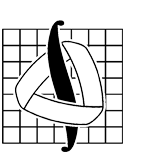
\includegraphics[width=20mm]{mmlogo.png}}
			\end{center}
		\end{figure}
		
		\vspace{3cm}
		
		Реферат по истории математики\\
		{\bf Бернард Больцано <<Парадоксы бесконечного>>}
		
		\vspace{8cm}
		\begin{flushright}
			{\bfРаботу выполнил:}\\
			студент 4 курса Сибгатуллин Артур Петрович\\[0.5cm]
		\end{flushright}
		\vspace{1cm}
		
		\normalsize Москва, 2022
	\end{center}
\end{titlepage}


\tableofcontents

\newpage
\section{Краткая биография}

Бернард Больцано родился 5 октября 1781 года в городе Праге в семье выходца из Северной Италии.

В 1796 году поступил в Карлов университет в Праге, сначала изучал математику, философию и физику на факультете философии, с 1800 — теологию на факультете теологии, в 1804 году принял сан католического священника. В 1805 году получил новообразованную кафедру истории и философии религии и защитил докторскую диссертацию . В 1818 году избран деканом философского факультета. Труды периода до 1819 года в основном относятся к теологии и философии, в них оппонировал Канту, выступал против психологизма в логике и чёткое разграничение логического и психологического.

Свободомыслие Больцано вызвало раздражение церковных властей, Папа римский потребовал у австрийского императора сместить Больцано. В 1820 году решением императора Больцано был снят со всех постов в университете и взят под надзор полиции. Больцано уехал в деревню и посвятил себя математике и логике.

В 1843 году Больцано заболел воспалением легких в тяжёлой форме. Осенью 1848 года его состояние ухудшилось, и 18 декабря 1848 года он умер в пражской больнице. 
\begin{center}
\bfseries Научная деятельность 
\end{center}


При жизни Больцано опубликовал только пять небольших работ по математике и несколько анонимных философских трактатов. Они значительно опередили научный уровень того времени и не привлекли внимания научной общественности. Только в конце XIX века, когда эти идеи независимо переоткрыли Вейерштрасс и Дедекинд, историки обнаружили и оценили по заслугам сочинения Больцано, и прежде всего его строгое обоснование математического анализа, построенное в работе <<Чисто аналитическое доказательство теоремы, что между любыми двумя значениями, дающими результаты противоположного знака, лежит по меньшей мере один вещественный корень уравнения>>. Больцано также на четыре года раньше Коши и более строго, чем он, вывел необходимое условие сходимости вещественных рядов.

В работе 1830 года Больцано нашёл первые примеры непрерывных нигде не дифференцируемых функций.

В труде <<Наукоучение>> (1837, нем. Wissenschaftslehre) представил объемлющее изложение традиционных логических учений.

Его работа <<Парадоксы бесконечного>> (нем. Paradoxien des Unendlichen) будет подробно рассмотрена далее.

\section{История вопроса}
Множества, в том числе и бесконечные, в неявной форме фигурировали в математике со времён Древней Греции: например, в том или ином виде рассматривались отношения включения множеств всех рациональных, целых, натуральных, нечётных, простых чисел. Зачатки идеи о равномощности множеств встречаются у Галилея: рассуждая о соответствии между числами и их квадратами, он обращает внимание на неприменимость аксиомы <<целое больше части>> к бесконечным объектам.

Первое представление об актуально бесконечном множестве относят к работам Гаусса начала 1800-х годов, опубликованным в его <<Арифметических исследованиях>>, в которых, вводя сравнения на множестве рациональных чисел, он обнаруживает классы эквивалентности (классы вычетов) и разбивает всё множество на эти классы, отмечая их бесконечность и взаимное соответствие. В более поздних работах Гаусс, рассматривая совокупность комплексных чисел с рациональными вещественной и мнимой частью, говорит о вещественных, положительных, отрицательных, чисто мнимых целых числах как её подмножествах. Однако бесконечные множества или классы как самостоятельные объекты исследования Гауссом явно не выделялись, более того, Гауссу принадлежат высказывания против возможности использования актуальной бесконечности в математических доказательствах.

Более отчётливое представление о бесконечных множествах проявляется в работах Дирихле, в курсе лекций 1856—1857 годов, построенном на основе гауссовых <<Арифметических исследований>>. В работах Галуа, Шёмана и Серре по теории функциональных сравнений 1820—1850-х годов также намечаются элементы теоретико-множественного подхода, которые обобщил Дедекинд в 1857 году, явно сформулировавший в качестве одного из выводов необходимость рассмотрения целой системы бесконечно многих сравнимых чисел как единого объекта, общие свойства которого равным образом присущи всем его элементам, а систему бесконечно многих несравнимых классов уподобляет ряду целых чисел. Отдельные понятия теории множеств можно встретить в трудах Штейнера и Штаудта 1830—1860-х годов по проективной геометрии: практически весь предмет в значительной степени зависит от представления о взаимно-однозначном соответствии, ключевом для теории множеств, однако в проективной геометрии на такие соответствия накладывались дополнительные ограничения (сохранение некоторых геометрических соотношений). В частности, Штейнер явно вводит понятие несчётного множества для множества точек на прямой и множества лучей в пучке и оперирует с их несчётными подмножествами, а в работе 1867 года вводит понятие мощности как характеристики множеств, между которыми возможно установить проективное соответствие.

Наиболее близкие к наивной теории множеств Кантора представления содержатся в трудах Больцано, прежде всего, в работе <<Парадоксы бесконечного>>, опубликованной в 1851 году, в которой рассматриваются произвольные числовые множества, и для их сравнения явно определено понятие взаимно-однозначного соответствия, и сам термин <<множество>> также впервые систематически использован в этой работе. 


\section{Предисловие}
\subsection{От редактора перевода}
Редактором перевода является профессор И.В.Слешинский. 

Он обращает внимание на то, что в венской библиотеке хранятся не опубликованные рукописи Больцано. Они составляют десять кип, и только одна не имеет отношения к математике. 

Больцано первым ввел в математику понятие о верхней границе, установил понятие о сходимости рядов, опередив в этом Коши, и сформулировал критерий сходимости.

В сочинении <<Парадоксы бесконечного>> Больцано является предшественником Георга Кантора в теории бесконечных многообразий. Именно он устанавливает и развивает свойства бесконечного, которые легли в основание теории Кантора.

Слешинский отмечает, что некоторые утверждения Больцано, которые касаются метафизики, оказались неверными, но мнения разделялись наиболее знаменитыми математиками той эпохи. При этом для понимания математических частей сочинения достаточно элементарных знаний из области высшей математики.

\subsection{От издателя}
Свое сочинение <<о парадоксах бесконечного>> Больцано начал писать еще летом 1847-го года, но закончил он его только летом последнего года своей жизни, так как должен был сделать перерыв для других работ. Этим сочинением он доказал, что несмотря на поздний возраст и упадок телесных сил, его духовные силы сохранили всю свежесть и подвижность.
Кроме того, эта работа показала всему ученому миру всю самобытность его воззрений на самые отвлеченные и глубокие вопросы математики, чистого естествознания и метафизики.

Издатель принял на себя обязательство напечатать трактат тем охотнее, что оно согласовалось с его желанием, так как Больцано был его учителем и другом. Для издания был выбран Лейпциг, потому что издатель надеялся на более широкое распространение сочинения и на то, что Лейпциг прославится тем, что был местом, где впервые появились <<Парадоксы>>. 

\newpage
\section{\S 1 - \S 10}
Понятие бесконечного выводится из понятия конечного путем присоединения к нему новой составной части. И понятие конечного, и понятие бесконечного относятся к многообразиям, к количествам (т.е. многообразиям единиц), рассматривают в науке в величинах -- математике, где рассматривают конечные и бесконечные множества и даже делают предметом вычисления бесконечных множеств наряду с конечными. 

Определим понятие, лежащее в основе союза \textit{\bf и}, следующим образом: \textit{Совокупность известных вещей или целое, состоящее из известных вещей}.

Любая вещь A с любыми вещами B, C, D... может составить совокупность вещей, или сама по себе составляет совокупность, о которой можно высказать
много истин, поскольку представления A, B, C, D... в действительности соответствуют различным предметам, т.е. поскольку ложно каждое из
следующих предложений: А есть то же, что В; А есть то же, что С; В есть то же, что С; и т.д. Если бы, например, А было тоже самое, что и В, то конечно было бы нелепым говорить о совокупности вещей А и В.

Назовем \textit{существенно различными} те совокупности, которые заключают те же части 
А, B, C, D..., но являются различными в зависимости от точки зрения(\textit{понятия}), с которой мы их рассматриваем. То, что лежит в основании различия таких совокупностей, мы называем \textit{способом соединения} их частей.
Если расположение частей при некотором понятии безразлично, то такую совокупность назовем \textit{многообразием}; а такое
многообразие, все части которого будут рассматриваться как
\textit{единицы} известного рода А, т.е как предметы, содержащиеся в
понятии А, называется \textit{множеством} предметов A.

Известно, что существуют совокупности, части которых являются
также составными, т.е. представляют из из себя опять совокупности.
Между ними есть также совокупности, которые мы рассматриваем с такой
точки зрения, что в них не произойдет существенного изменения, если мы
станем рассматривать части частей, как части целого. Этого рода
совокупности будем называть термином заимствованным у математиков, –
\textit{суммами}.

Предмет, любые две части \textit{M} и \textit{N} которого не могут никогда иметь другого отношения между собой, как равенство или одна из них является суммой,  содержащаю часть равную другой, т.е., что или $M = N$, или $M = N + \nu$, или $N = M + \mu$; причем для $\nu$ и $\mu$ имеет место тоже самое.

Пусть данная совокупность предметов A, B, C, D, E, F . . . . L, M, N... обладает таким свойством, что для каждой части M можно указать одну и только одну часть N такую, что с помощью закона одинакового для всех частей совокупности можно определить, – или N его отношением к M, или M его отношением к N, – то такое собрание называется \textit{рядом}, а части его \textit{членами} этого ряда. Закон, по
которому или N определяется отношением к M, или M отношением к N,
назовем \textit{законом составления ряда}. Один из членов ряда, притом какой угодно, назовем \textit{предыдущим} 
другой – \textit{последующим} (не обозначая этим названием
действительной последовательности во времени или пространстве). \textit{Внутренним} членом ряда назовем каждый член M, который имеет предыдущий член и последующий, т.е. не только сам получается из
другого члена, но и от которого тоже получается третий член, по закону
составления этого ряда. Отсюда понятно, какой член называть \textit{внешним}, \textit{первым} и \textit{последним}.

Рассмотрим \textit{ряд}, первый член которого есть
единица рода A, а каждый \textit{последующий} член составляется из своего \textit{предыдущего} таким образом, что, взяв предмет ему равный, соединяют его с новой единицей рода A, образуя из них сумму. Тогда все входящие в этот ряд члены, за исключением первого, который
представляет \textit{простую единицу} рода A, будут количествами.
Они будут представлять именно те количества, которые называют
\textit{конечными} или \textit{исчислимыми количествами}
или даже – со включением первого члена – \textit{числами} , более
определенно: \textit{целыми} числами. То есть строится аналог аксиоматики Пеано (возможно, именно это сочинение легло в основу его теории).

Смотря по различным свойствам понятия, которое обозначено через A, оно может заключать в себе то большее, то меньшее количество предметов, т.е. единиц рода A; поэтому в ряде может быть и большее и меньшее количество членов. Их может быть также столько, что ряд, который должен исчерпать все эти единицы, не будет иметь \textit{последнего члена}, это будет доказано впоследствии. Установив это, назовем
\textit{бесконечным количеством} количество большее, чем
каждое конечное, т.е. количество такого рода, что каждое конечное
многообразие представляет только часть его.

Если бы оказалось, что понятие бесконечного в настоящем значении слова может быть применено только к количествам, т.е., что бесконечность есть
свойство одних только количеств, то данное ранее определение бесконечных количеств было бы определением бесконечности. По мнению Больцано это действительно справедливо. Математик не употребляет никогда этого слова в другом смысле, так как он занимается почти исключительно определением величин, принимая одну из них за единицу и пользуясь понятием о
числе. Если он находит величину, которая больше, чем любое число тех
которые приняты за единицу, то он называет ее \textit{бесконечно большой}. Если же он находит величину столь малую, что каждое
кратное ее оказывается меньше единицы, то он называет ее
\textit{бесконечно малой}. Кроме этих двух родов бесконечного и
кроме выводимых из них родов бесконечно больших и бесконечно малых
\textit{величин высшего поярдка}, которые вытекают все из того
же понятия, для математика не существует ничего бесконечного.

\section{\S 11 - \S 20}
Некоторые определения бесконечности, которые были даны другими математиками Больцано опровергает в \S 12. 
Коши описывал бесконечность как переменную величину, которая возрастает безгранично, то есть может сделаться больше всякоц данной величины. Но это определение ошибочно, потому что переменной величиной математики называют не саму величину, а только представление о ней. 
И если это определение слишком широко, то другие философы и математики взяли за основу слишком узкое определение: только то бесконечно, что не способно к дальнейшему увелечению. Но математик позволяет себе прибавлять к каждой величине и для него это определение некорректно. 
Третье определение утверждает, что бесконечность есть то, что не имеет конца. Но если при этом иметь в виду конец во врмени, то неясно как это определение применить к другим вещам. Если же понимать это слово в более широком смысле, например, в смысле границы, то во-первых, существуют конечные предметы, для которых нельзя явным образом указать границу, а во-вторых, существует множество предметов ограниченных, но рассматриваемых как величины бесконечные. 

Как только мы пришли к соглашению, какое понятие мы должны связывать со словом \textit{бесконечный} , и как только мы уяснили себе вполне составные части этого понятия, то ближайшим вопросом является следующий: обладает ли это понятие \textit{предметностью}, то есть существуют ли предметы, к которым оно применимо, многообразия, которые мы можем назвать бесконечными в установленном нами значении. На этот вопрос можно смело ответить утвердительно. Очень легко заметить, что многообразие предложений и истин самих в себе -- бесконечно. Например, если мы станем рассматривать какую-нибудь истину, скажем, что истины вообще существуют, или любую другую истину, которую мы обозначим через A, то мы увидим, что предложение, выраженное словами <<A истинно>>, уже отлично от A, потому что предложение A имеет, очевидно, совершенно другое подлежащее. Далее, по тому самому закону, по которому мы вывели из предложения A отличное от него предложение, которое мы назовем B, мы можем вывести из B третье предложение C, и так далее без конца. Совокупность всех этих предложений, из которых каждое последующее находится к непосредственно предыдущему в только что указанном отношении, а именно, что подлежащим последующего предложения является предыдущее предложение, о котором высказывается, что оно истинно, эта совокупность обнимает такое многообразие частей (предложений), которое больше, чем всякое конечное многообразие. Ибо нетрудно заметить сходство, которое имеет ряд предложений, составленных по только что приведенному закону образования с рядом чисел, который был рассмотрен ранее.

Противники этой теории утверждают, что бесконечного множества не может быть нигде потому, что бесконечное не может быть соединено в одно целое и не может быть объято целиком в <<мысли>>. Ошибка этого убеждения состоит в том, что для того, чтобы вообразить себе целое, состоящее из известных предметов, нужно сперва составить представление о каждом отдельном предмете. Но мы можем вообразить себе множество всех жителей крупного города, не представляя каждого жителя в отдельности.

Существует еще одно ошибочное мнение, что <<многообразие не существовало бы, если бы не было кого-то, кто думал о нем>>. В качестве контрпримера Больцано приводит физические законы, которые выполняются независимо от того, думает о них кто-либо или нет.

Некоторые говорят: <<Для того чтобы существовала
совокупность, нет надобности в том, чтобы мыслящее существо
действительно думало о ней, но необходимо, чтобы о
ней можно было думать. А так как мыслящее существо не может
представить себе бесконечное множество вещей, каждую в отдельности, и
связать затем эти представления в совокупность, то невозможна и
совокупность, заключающая в себе бесконечное множество вещей в
качестве составных частей>>. Ранее было показано, что это утверждение ошибочно, но хотелось бы подчеркнуть еще несколько мыслей Больцано об этой проблеме.

Мы не должны соглашаться с тем, что существование совокупности вещей покоится на возможности думать об этой совокупности. Ибо возможность мыслить вещь не составляет основания для возможности ее существования. Напротив того, возможность существования вещи составляет основание для того, чтобы разумное существо, если оно только не впадает в ошибку, нашло эту вещь возможной, т.е. чтобы ее можно было мыслить. Мы убедимся вполне в правильности этого замечания и в полной несостоятельности очень распространенного мнения, которое здесь оспаривается, если постараемся уяснить себе составные части важного понятия "возможности". Если называют \textit{возможным} то, что может быть, то это, очевидно, еще не будет разложение понятия о возможности, так как оно заключается целиком в выражении "может быть". Но еще неправильнее было бы пытаться установить следующее определение: возможно то, что можно мыслить. Мыслить, в собственном значении этого слова, включая сюда уже и простое представление , мы можем и невозможное. Это мы и делаем в действительности каждый раз, когда мы высказываем о нем суждение, – признаем его, например, невозможным.

Ранее было доказано, что существуют бесконечные множества, по крайней мере, среди вещей нериальных, а именно, что множество всех истин в себе бесконечно. Аналогично тому, как это было сделано мы докажем, что множество всех чисел бесконечно. Это положение будем считать \textit{первым} среди парадоксов, появляющихся в области математики.

<<Если каждое число>> есть лишь простое конечное множество, то каким образом может быть бесконечным множество всех чисел? Когда мы рассматриваем ряд натуральных чисел $1,\, 2,\, 3,\, 4,\, 5,\, 6, \ldots$ то мы замечаем, что множество чисел, которое содержит этот ряд, начиная с первого, до какого-нибудь другого, например, до числа 6, выражается всегда этим последним числом. Поэтому множество всех чисел должно быть так велико, как \textit{последнее} из них и, следовательно, само должно быть числом, а не бесконечностью». Обманчивость этого вывода исчезает тотчас же, как только мы вспомним, что во множестве всех чисел в натуральном ряду нет последнего числа, что таким образом понятие о последнем числе – понятие беспредметное, потому что содержит противоречие. Ибо, по закону образования этого ряда, каждый член ряда имеет \textit{последующий}. Одним этим замечанием разрешается этот
парадокс.

\textit{Время и пространство} представляют в высшей степени важный род бесконечно больших величин, которые также еще не принадлежат к области реального, хотя и могут определять реальное. Ни время, ни пространство не представляют ничего реального, так как они не представляют из себя ни \textit{субстанций}, ни свойств субстанций. Они выступают только, как нечто определяющее для всех несовершенных (ограниченных,
конечных или, что сводится к одному и тому же, зависимых, сотворенных)
субстанций, а именно, каждая из последних должна постоянно пребывать в некотором времени и известном пространстве, таким образом, что каждая простая субстанция в каждом пункте времени, т.е. в каждой простой части времени должна пребывать в какой-нибудь простой части пространства, т.е. в какой-нибудь его точке. Множество простых частей или точек, из которых состоит время и пространство, бесконечно. Бесконечно не только количество простых частей, из которых состоит все время и все пространство, т.е. количество точек времени и пространства вообще, но и количество точек времени (пространства) между двумя точками a и b, как бы близко ни отстояли эти точки друг от друга, тоже бесконечно.

Хотя каждая величина которая нам представляется бесконечной в каком-либо отношении, должна представляться нам именно в этом отношении, как целое, состоящее из бесконечного множества частей, – невозможно однако утверждать обратное, чтобы каждая величина, которую мы рассматриваем, как сумму бесконечного множества других конечных величин, была бесконечной. Например сумма бесконечного ряда слагаемых может быть конечным числом
$$
a + ax + ax^2 + ax^3 + \ldots = \sum_{i = 0}^{\infty} ax^i = \frac{a}{1-x} \mbox{, при } e < 1.
$$

Следующий рассматриваемый парадок заключается в том, что мы можем построить взаимооднозначное соответствие между двумя бесконечными многообразиями, но при этом одно многообразие будет являться частью другого. Например, множество натуральных и четных чисел:
$$
\begin{array}{c c c c c c c c c c c c c c c c}
1 & 2 & 3 & 4 & 5 & 6 & 7 & 8 & 9 & 10 & 11 & 12 & 13 & 14 & 15 & \ldots \\
\updownarrow &
\updownarrow &
\updownarrow &
\updownarrow &
\updownarrow &
\updownarrow &
\updownarrow & 
\updownarrow &
\updownarrow &
\updownarrow &
\updownarrow &
\updownarrow &
\updownarrow &
\updownarrow &
\updownarrow & \\
2 & 4 & 6 & 8 & 10 & 12 & 14 & 16 & 18 & 20 & 22 & 24 & 26 & 28 & 30 & \ldots
\end{array}
$$

\textit{Сам Бернард Больцано предлагает в качестве примера следующую конструкцию:}

Рассмотрим две величины, например, $5$ и $12$. Ясно, что многообразие величин между $0$ и $5$ (а также между $0$ и $12$) бесконечно.
Также ясно, что второе многообразие должно считаться большим, чем первое. Пусть $x \in [0; 5]$. Определим соотношение между $x$ и $y$ уравнением $5y = 12x$. Отсюда следует, что $y \in [0; 12]$. И наоборот, если $y$ содержится между $0$ и $12$, то $x$ лежит между $0$ и $5$. Из этого же уравнения следует, что каждому значению $x$ соответствует ровно один $y$. Верно и обратное. Это значит, что для каждого элемента первого многообразия есть \textit{парный} элемент из второго и наоборот, но второе многообразие больше первого. 

\section{\S 21 - \S 30}

Только на том основании, что два многообразия $A$ и $B$ находятся друг к другу в таком отношении, что к каждой части $a$, находящейся в $A$, поступая по известному правилу, мы можем найти находящуюся в $B$ часть $b$, так, что все пары $(a + b)$, которые мы составим таким образом, заключают в себе каждую вещь, находящуюся в $A$ и в $B$ и заключают ее только по одному разу, – на одном только этом основании невозможно еще заключить, как видим, что эти оба многообразия, если они бесконечны равны друг другу  в отношении множества своих частей (т.е. если мы не примем во внимание никаких других различий между частями). 
Однако, несмотря на это отношение между ними, которое само по себе, представляется одинаковым для обоих многообразий, они могут находиться в отношении неравенства своих множеств, так что одно из них может представлять целое, а другое – его часть. О равенстве этих множеств можно будет заключить только тогда, когда для этого будет существовать еще какое-нибудь другое основание, как, например, то, что оба многообразия имеют совершенно одинаковые определяющие их основания, например, совершенно одинаковое происхождение.

Если мы можем считать доказанным и разъясненным предложение \S 20, то  его следствиемявляется то, что мы не можем считать равными две суммы величин, которые попарно равны(т.е. каждая величина из одной суммы равна некоторой величине из другой), если множество их бесконечно. 
Это возможно лишь в том случае, когда мы заранее убедились в том, что бесконечное множество этих величин в обеих суммах то же самое. Что сумма определяется своими слагаемыми и что равные слагаемые дают равные суммы, это конечно бесспорно и имеет место не только тогда, когда многообразие этих слагаемых конечно, но и тогда, когда оно бесконечно. 
Но, так как бесконечные многообразия бывают различны, то в последнем случае должно быть также доказано, что бесконечное многообразие слагаемых в одной сумме в точности таково же, как и в другой. Но, чтобы иметь право сделать это заключение, недостаточно ни в каком случае, по нашей теореме, только того обстоятельства, что можно будет найти по какому-нибудь способу для каждого члена одной суммы равный ему член другой суммы. Мы можем сделать это заключение с полной уверенностью только тогда, когда оба эти многообразия имеют одинаковые определяющие их основания.

Больцано признает, что если раньше он имел смелость защищать существование бесконечности с некоторых случаях против лиц, оспаривающих его, то с той же откровенностью он признает, что некоторые ученые математики зашли слишком далеко в определении \textit{бесконечно большого} и \textit{бесконечно малого} в случаях, когда ни того, ни другого не существует.

Под бесконечно большим периодом времени можно понимать период, не имеющий начала или конца (или ни того, ни другого), но отношение, которое имеет величина одного расстояния между точками к другому, может быть только конечным.

То же самое можно сказать о расстояниях в пространстве, которые могут быть друг ко другу всегда только в отношении конечном.

Установленные ранее правила дадут нам возможность правильно судить о всех странных учениях, которые мы будем рассматривать далее.

Рассмотрим сумму натуральных чисел:
$$
1 + 2 + 3 + \ldots + n + (n+1) + \ldots
$$
При этом выражение 
$$
1^0 + 2^0 + 3^0 + \ldots + n^0 + (n+1)^0 + \ldots
$$
будет являться количеством натуральных чисел. Обозначим его через $N^0$ и подобным образом обозначим количество чисел от $(n+1)$ через $N^n$, то мы получим прекрасное равенство: 
$$
1^0 + 2^0 + 3^0 + \ldots + n^0 = N^0 - N^n
$$
из которого видно, что две бесконечные виличины имеют конечную разность.

Умножим обе части равенства: 
$
1^0 + 2^0 + 3^0 + \ldots + n^0 + (n+1)^0 + \ldots = N^0
$
на $N^0$, получим:
$$
1^0 \cdot N^0 + 2^0 \cdot N^0 + 3^0 \cdot N^0 + \cdots + n^0 \cdot N^0 + (n+1)^0 \cdot N^0 + \cdots = {(N^0)}^2
$$
и т.д. Из этого мы видим, что существуют бесконечные величины, так называемых \textit{высших порядков}, из которых одна превосходит другую в бесконечное число раз.

Эти примеры в достаточной степени показывают, что существует исчисление бесконечно большого, а тогда и бесконечно малого, так как мы можем рассмотреть, например, величину $\frac{1}{N^0}$. 

Далее вводится некоторый аналог дифференцирования. На примере равенства (которое можно рассматривать как функцию $y(x)$) вводятся малые изменения величин $x$ и $y$ и находится соотношение между этими малыми изменениями, то есть дифференциал функции $y(x)$.

\newpage
\section{Заключение}
Математические парадоксы являются одной из самых интересных тем для изучения. Понятие бесконечности с одной стороны является довольно интуитивным, а с другой очень неоднозначным понятием. При этом эта тема интересна не только с точки зрения математики, но и философии. Именно поэтому для написания аннотации мною был выбран труд Б. Больцано "Парадоксы бесконечного".

Больцано предельно ясно излагает свои взгляды, предоставляет доступные для понимания доказательства. При этом требуются только элементарные знания из области высшей математики. Нельзя не согласиться со словами издателя, относящимися к Больцано: "Самые интересные и запутанные вопросы, возникающие при исследовании понятия о бесконечности, вопросы, которые занимали с давних времен ученых, работавших в области априорных наук, он умеет разрешать с поразительной легкостью." 

Больцано различал актуальную и потенциальную бесконечность. Под актуальной бесконечностью он понимал "количество большее, чем каждое конечное, т.е. количество такого рода, что каждое конечное многообразие представляет только часть его". Он исследовал свойства актуальной бесконечности. Потенциальная бесконечность определяется из следующего высказывания Больцано "я присоединяюсь к тем, кто находится в отрицательном отношении к этому понятию о величине, которая только бесконечно возрастает, но никогда не достигает бесконечности."

В своем последнем сочинении <<Парадоксы бесконечного>> Больцано отчётливо показывает законность и существенную необходимость понятия актуальной бесконечности. При этом он значительно приумножает число парадоксальных следствий, которые при желании могут быть извлечены из этого понятия. Он показывает чисто иллюзорную природу так называемых противоречий, которые возникают вследствие неправильного определения бесконечного, а также неправильного понимания исчисления бесконечного. Больцано разработал теорию бесконечных величин, дал бесконечной величине определение, указал на возможность ее исчисления, применил бесконечную величину в геометрии, разработал ее свойства и привел доказательства своих взглядов.

Разрешая противоречия, Больцано ввёл понятие эквивалентности, которое в области бесконечного соответствует понятию равенства применительно к конечным числам и суммам. При этом он показал различие между равенством и эквивалентностью. Эквивалентность не включает в себя равенство: первое отношение имеет место в случае бесконечного, второе, наоборот, лишь в случае конечного.

В <<Парадоксах бесконечного>> были предвосхищены многие понятия теории бесконечных множеств. Он устанавливает и развивает те свойства бесконечного, которые легли в основание теории Кантора. Кроме того, Больцано даёт то определение суммы, на котором построит свою арифметику Г. Грассман; даёт научное определение нуля. Интересны его идеи, относящиеся к обоснованию метода исчисления бесконечного, а также к понятиям о времени и пространстве. 

Однако, работа Больцано носит в большей степени философский характер, нежели математический, в частности, в ней нет чёткого разграничения между мощностью множества и понятием величины или порядка бесконечности, и сколь-нибудь формальной и целостной математической теории в этих представлениях нет.

Тем не менее Бернард Больцано внес огромный вклад в историю и развитие теории множеств в современной математике.


\newpage
\begin{thebibliography}{99}
\bibitem{1} 
\textsc{Больцано Б.} Парадоксы бесконечного. Одесса, 1911
\end{thebibliography}
\end{document}